\subsubsection{Semi-supervised learning: leveraging real unlabeled resections}
\label{sec:results_semi}

\newcommand{\pseudo}{\st{pseudo}}

In this experiment, we assessed the ability of semi-supervised learning to improve the performance of our baseline model.
We first computed the uncertainty $u(f_{\alpha\beta}, \X\post, n\st{unc})$ for
$D\unl$ (\sectionref{sec:leveraging_semi}),
all unlabeled images in EPISURG,
%$D\st{R} = \{ \X_{\text{R}_i} \}_{i = 1}^{n\st{R}}$, where $n\st{R} = 297$ (\figureref{fig:uncertainties}),
using the baseline model and the preprocessing and augmentation transforms (\sectionref{sec:preprocessing_augmentation}).
%We generated pseudolabels using data distillation (\sectionref{sec:leveraging_semi}) for all images in $D\unl$
%with $u(\X_{\text{postop}_i}, \cdot) < t\st{unc} = 0.2$ (\figureref{fig:all_uncertainties}) to obtain the dataset
%$D\pseudo = \{ (\X_{\text{postop}_i}, \wt{\Y}_{\text{cavity}_i}) \}_{i = 1}^{n\pseudo}$, where $n\pseudo = 256$.
%We computed uncertainty and generated the pseudolabels from $n\st{unc} = 50$ Monte Carlo \ac{TTA} iterations (\figureref{fig:uncertainty_pseudo}).
%, where uncertainty and pseudolabels are generated from $n\st{unc} = 50$ Monte Carlo \ac{TTA} iterations.
We generated pseudolabels and estimated uncertainty from $n\st{unc} = 50$ Monte Carlo \ac{TTA} iterations (\sectionref{sec:leveraging_semi}).
To obtain the final dataset $D\pseudo = \{ (\X_{\text{postop}_i}, \wt{\Y}_{\text{cavity}_i}) \}_{i = 1}^{n\pseudo}$, we selected pseudolabels with $u(\X_{\text{postop}_i}, \cdot) < t\st{unc} = 0.2$, resulting in $n\pseudo = 256$.
% Explain why 0.2?

We used $D\st{pre,train}$ (\sectionref{sec:self}) in addition to $D\pseudo$ to train a new model $\fp{sim,semi}(\cdot)$, using the same hyperparameters as in the self-supervised setting (\sectionref{sec:self}).
To ensure that all batches contain real resections, we use $b - b\pseudo$ images from $D\st{pre,train}$ and $b\pseudo$ images from $D\pseudo$ to compose each mini-batch of size $b$.
We chose $b\pseudo = 2$ for our experiments, i.e., 20\% of the images in each mini-batch contain real resection cavities.

Semi-supervised learning improved the performance of the baseline model from 80.5 (18.7) to 81.5 (17.8) ($p = 0.474$).  % Experiment 37
%Although this difference was not statistically significant ($p = 0.474$), we note that this model was trained using no manual annotations.

% trim is "left bottom right top"

\newcommand{\uncertainties}[1]{
    \subfigure{%
        \includegraphics[trim=0 680 642 32, clip, width=0.25\linewidth]{#1_uncertainty}
        \includegraphics[trim=642 680 0 32, clip, width=0.25\linewidth]{#1_uncertainty}
        \includegraphics[trim=0 0 642 714, clip, width=0.25\linewidth]{#1_uncertainty}
        \includegraphics[trim=642 0 0 714, clip, width=0.25\linewidth]{#1_uncertainty}
    }
}

\newcommand{\uncertaintiescap}[1]{
    \subfigure{%
        \label{fig:uncertainty_mri}%
        \includegraphics[trim=0 680 642 32, clip, width=0.25\linewidth]{#1_uncertainty}
    }%
    \subfigure{%
        \label{fig:uncertainty_std}%
        \includegraphics[trim=642 680 0 32, clip, width=0.25\linewidth]{#1_uncertainty}
    }%
    \subfigure{%
        \label{fig:uncertainty_mean}%
        \includegraphics[trim=0 0 642 714, clip, width=0.25\linewidth]{#1_uncertainty}
    }%
    \subfigure{%
        \label{fig:uncertainty_pseudo}%
        \includegraphics[trim=642 0 0 714, clip, width=0.25\linewidth]{#1_uncertainty}
    }
}



% image - mean - std - pseudolabeled
% sid=0914
% scp -r dgx:/home/fernando/datasets/real/pseudo/image/$sid\* .
% scp -r dgx:/home/fernando/datasets/real/pseudo/label/$sid\* .
% scp -r dgx:/home/fernando/datasets/real/pseudo/aleatoric/std/$sid\* .
% scp -r dgx:/home/fernando/datasets/real/pseudo/aleatoric/mean/$sid\* .


% bien 0499
% regular 0914  # 568
% mal 0796

\begin{figure}[ht!]
    \centering
    \floatconts
    {fig:uncertainties}
    {\caption{%
        Generating reliable pseudolabels for semi-supervised learning.
        Image-level uncertainty for the 297 unlabeled postoperative images in EPISURG (a).
        Unlabeled postoperative \ac{T1} \ac{MRI} (b).
        Voxel-wise uncertainty (c) estimated as the standard deviation of the probabilities across all Monte Carlo iterations.
        The mean prediction (d) is thresholded at 0.5 to generate the pseudolabel (e).
        Image-level uncertainties for the three cases are 0.805 (top), 0.195 (middle) and 0.025 (bottom).
    }}
    {
        \subfigure{%
            \label{fig:all_uncertainties}%
            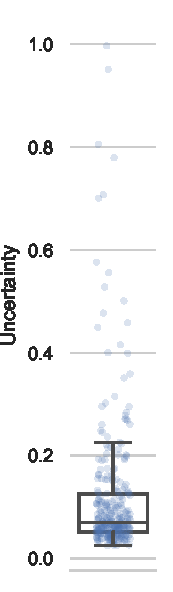
\includegraphics[width=0.15\linewidth]{qcd}
        }%
        \subfigure{%
            \label{fig:uncertainty_mri}%
            \begin{tabular}{c}
                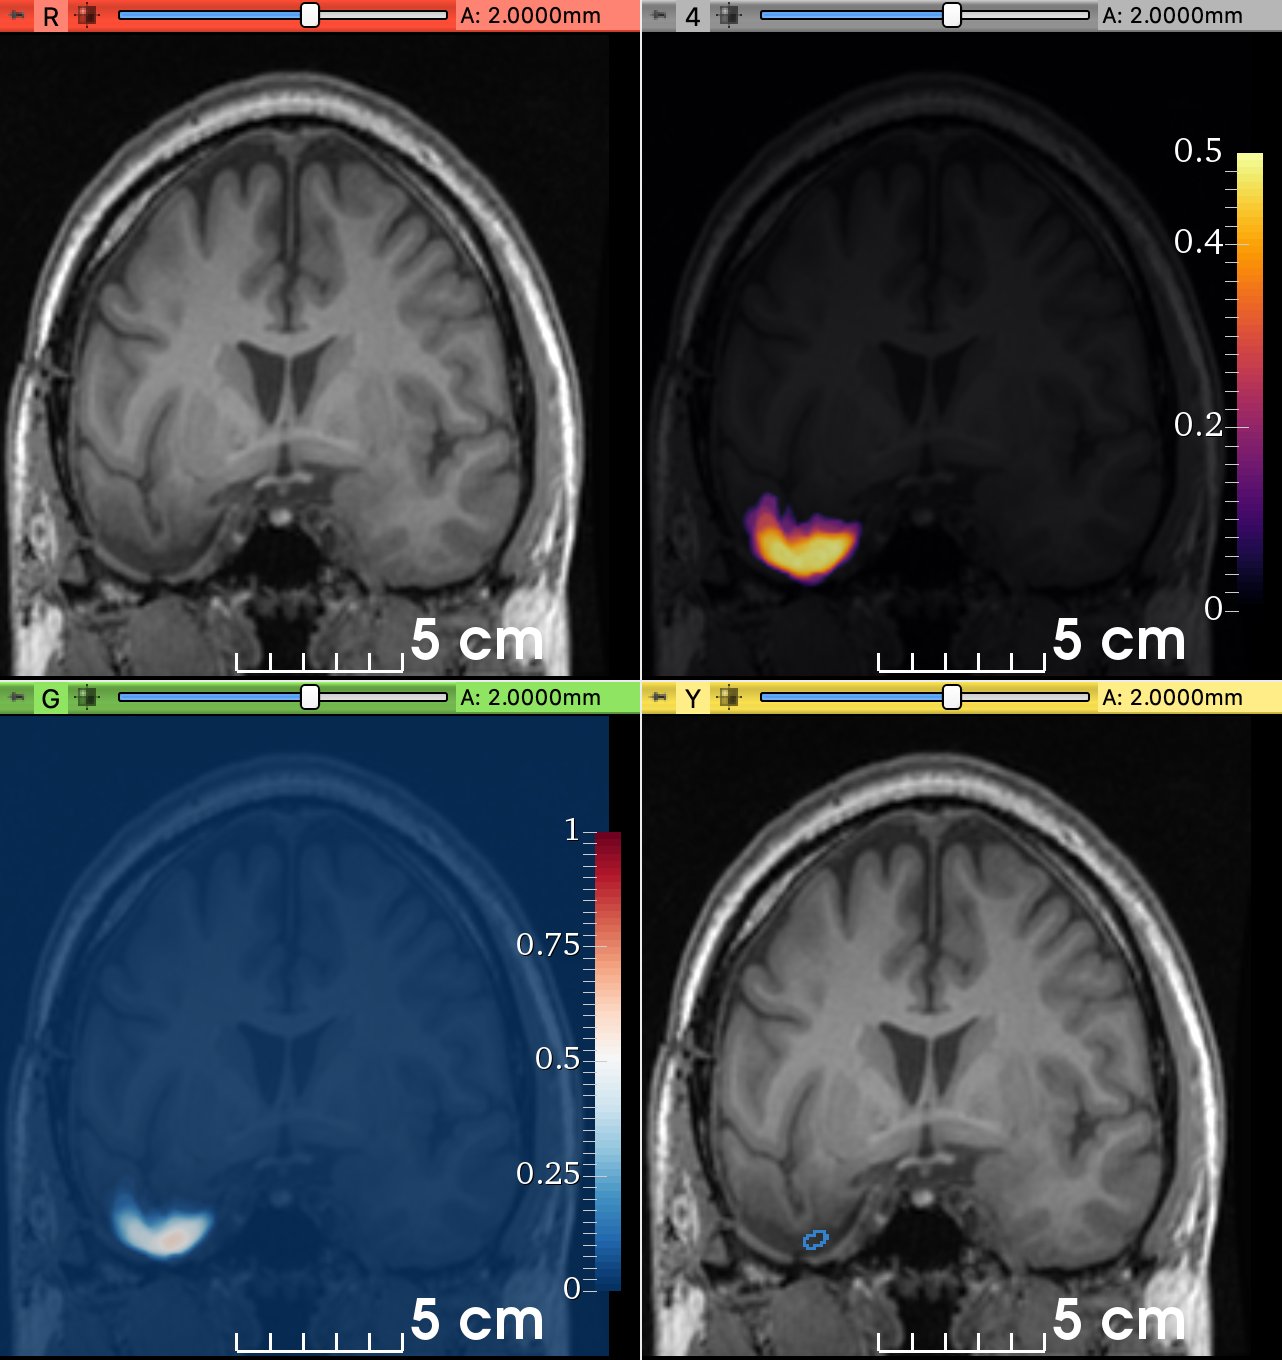
\includegraphics[trim=0 680 642 32, clip, width=0.15\linewidth]{0796_uncertainty} \\
                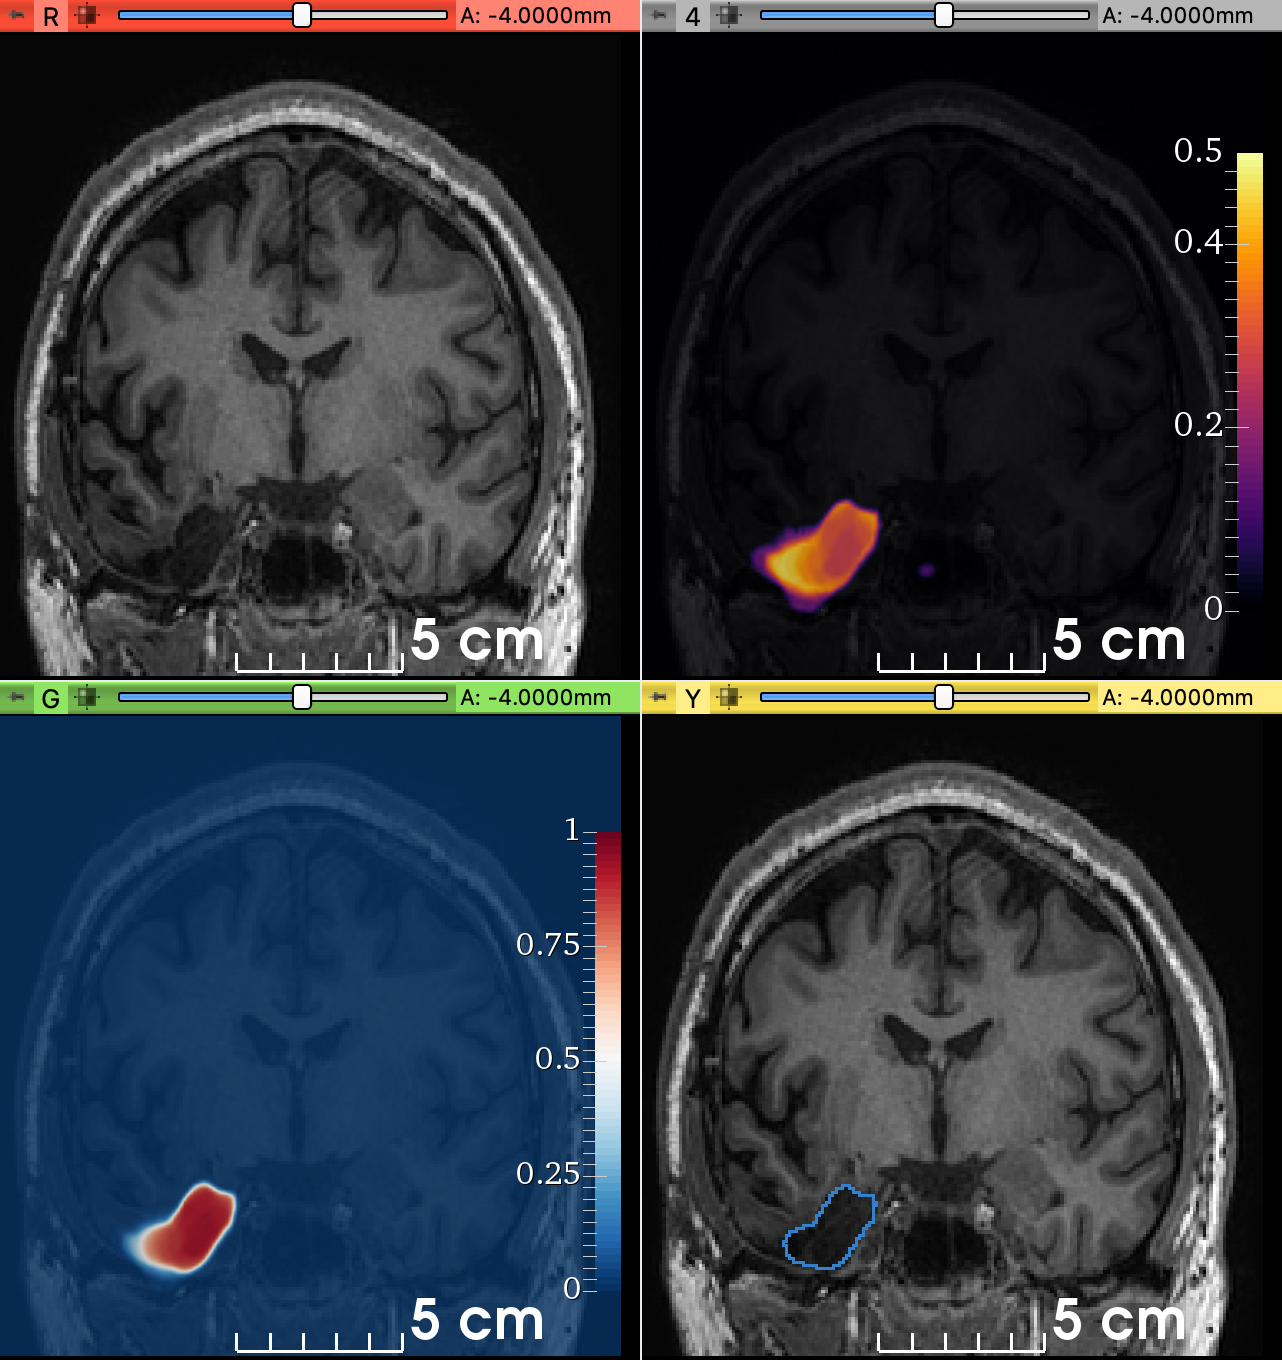
\includegraphics[trim=0 680 642 32, clip, width=0.15\linewidth]{0914_uncertainty} \\
                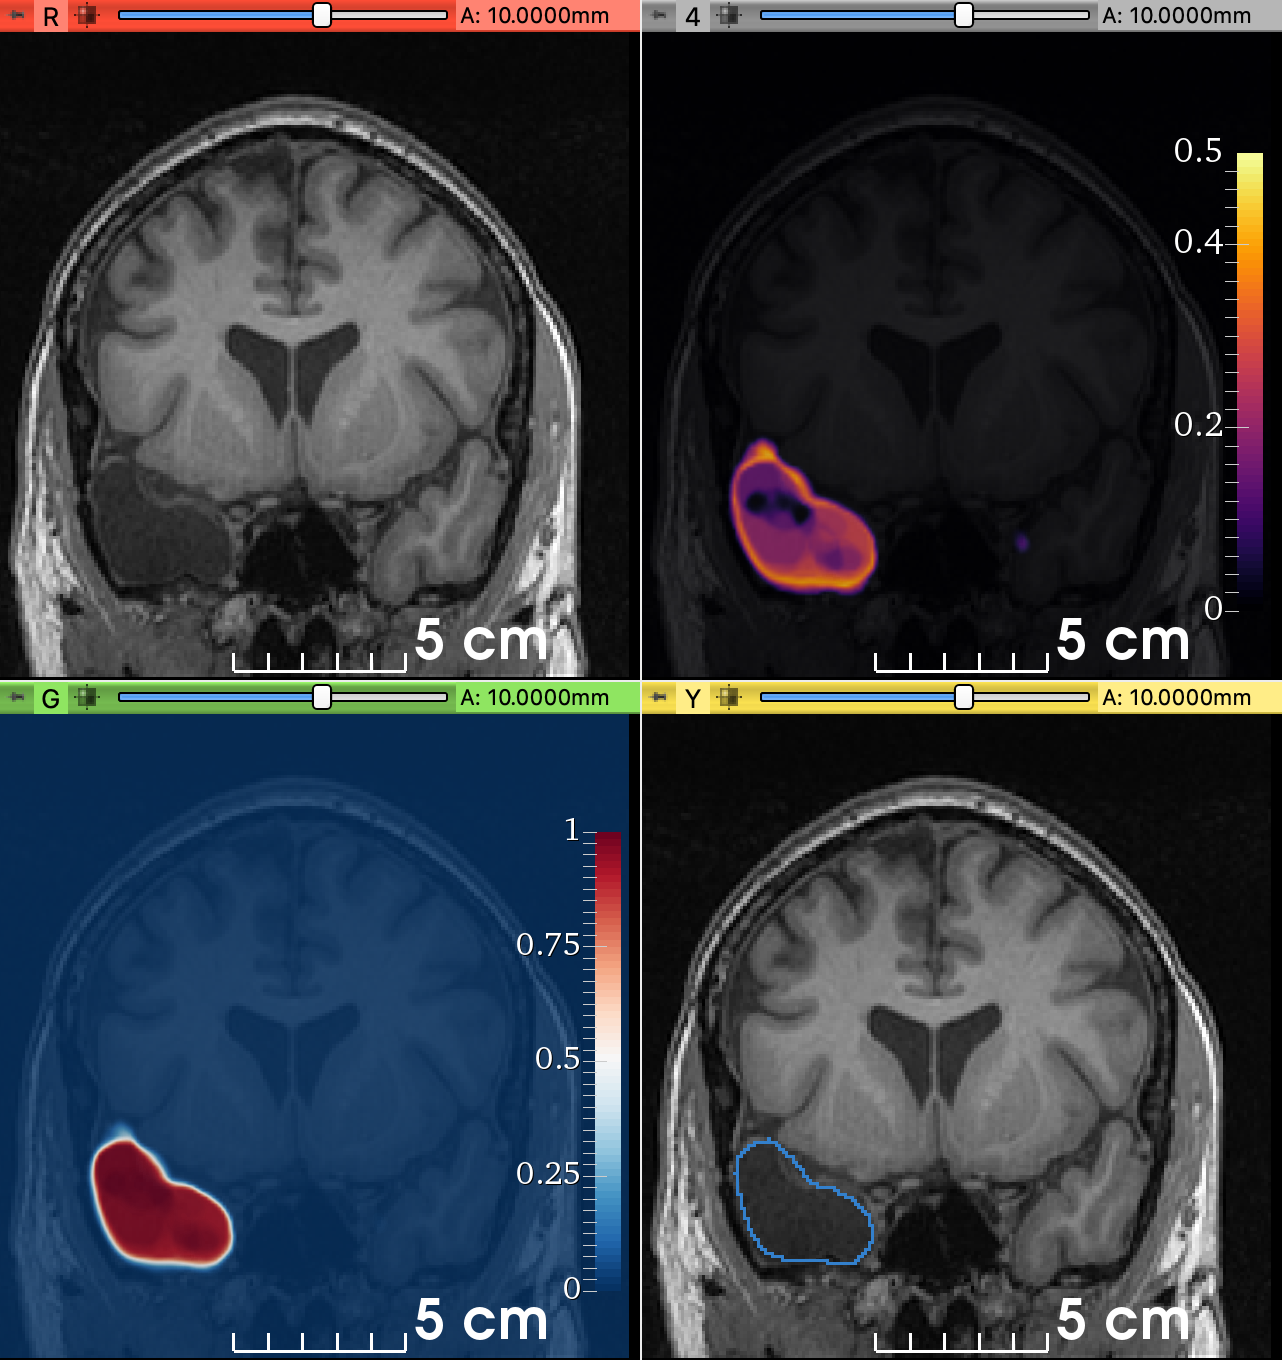
\includegraphics[trim=0 680 642 32, clip, width=0.15\linewidth]{0499_uncertainty} \\
            \end{tabular}
        }%
        \subfigure{%
            \label{fig:uncertainty_std}%
            \begin{tabular}{c}
                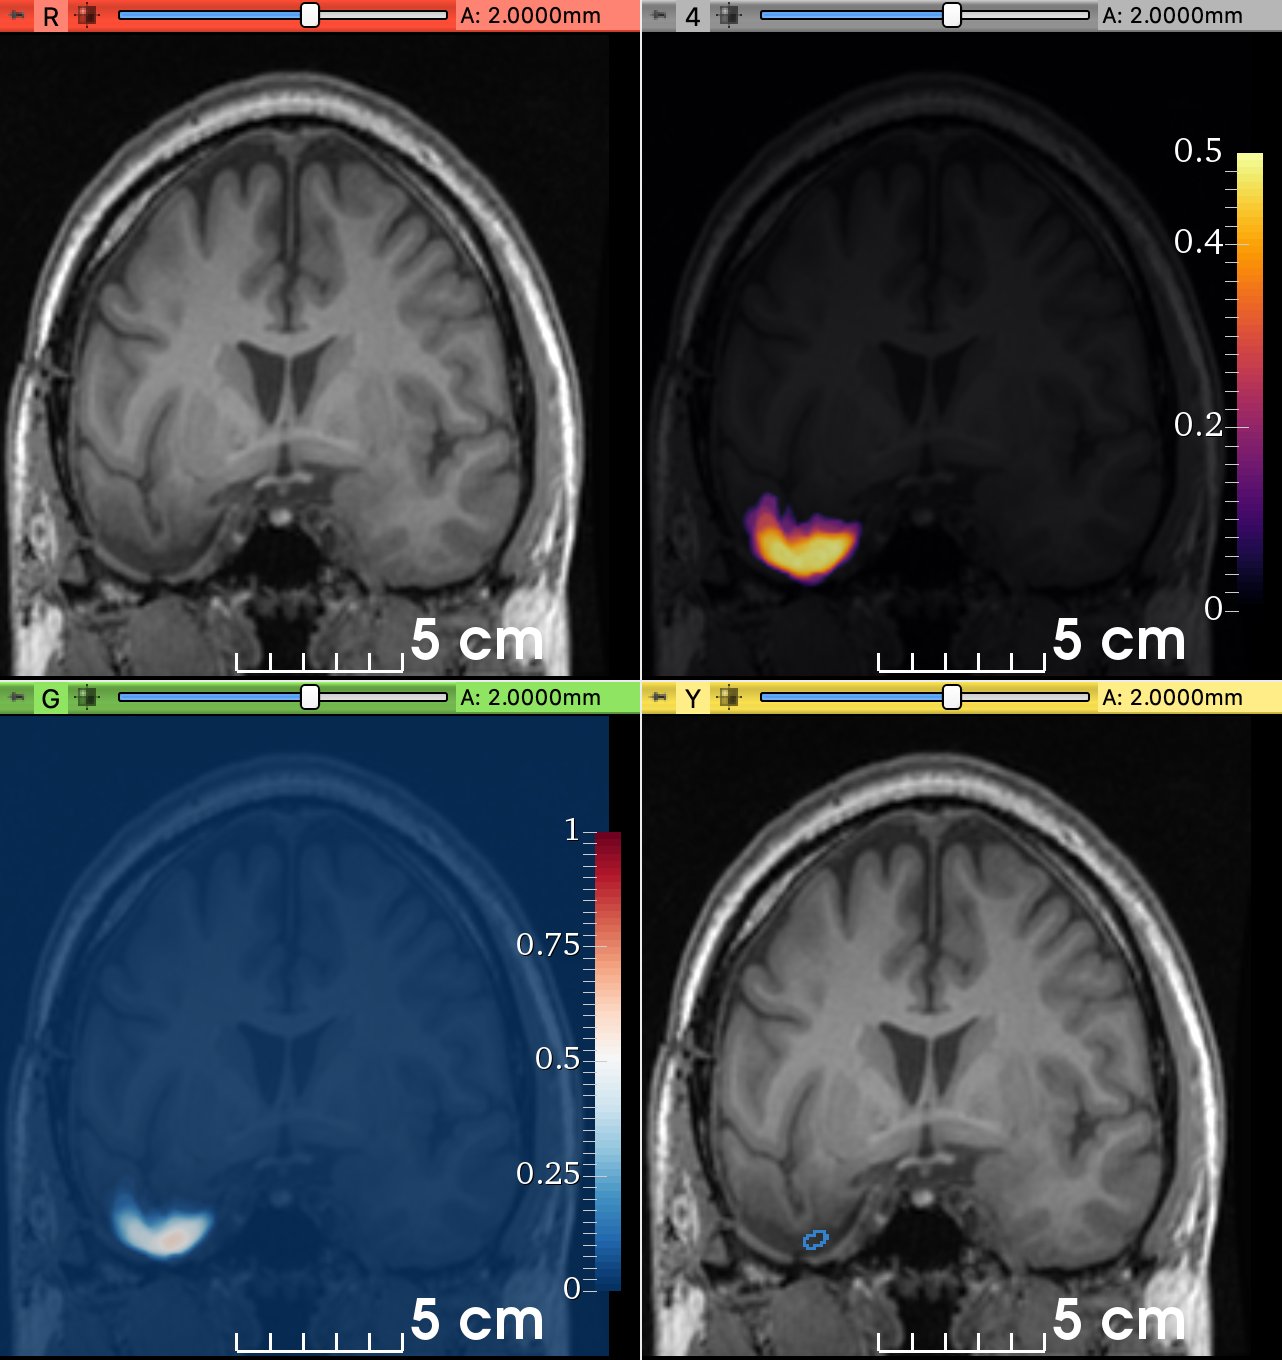
\includegraphics[trim=642 680 0 32, clip, width=0.15\linewidth]{0796_uncertainty} \\
                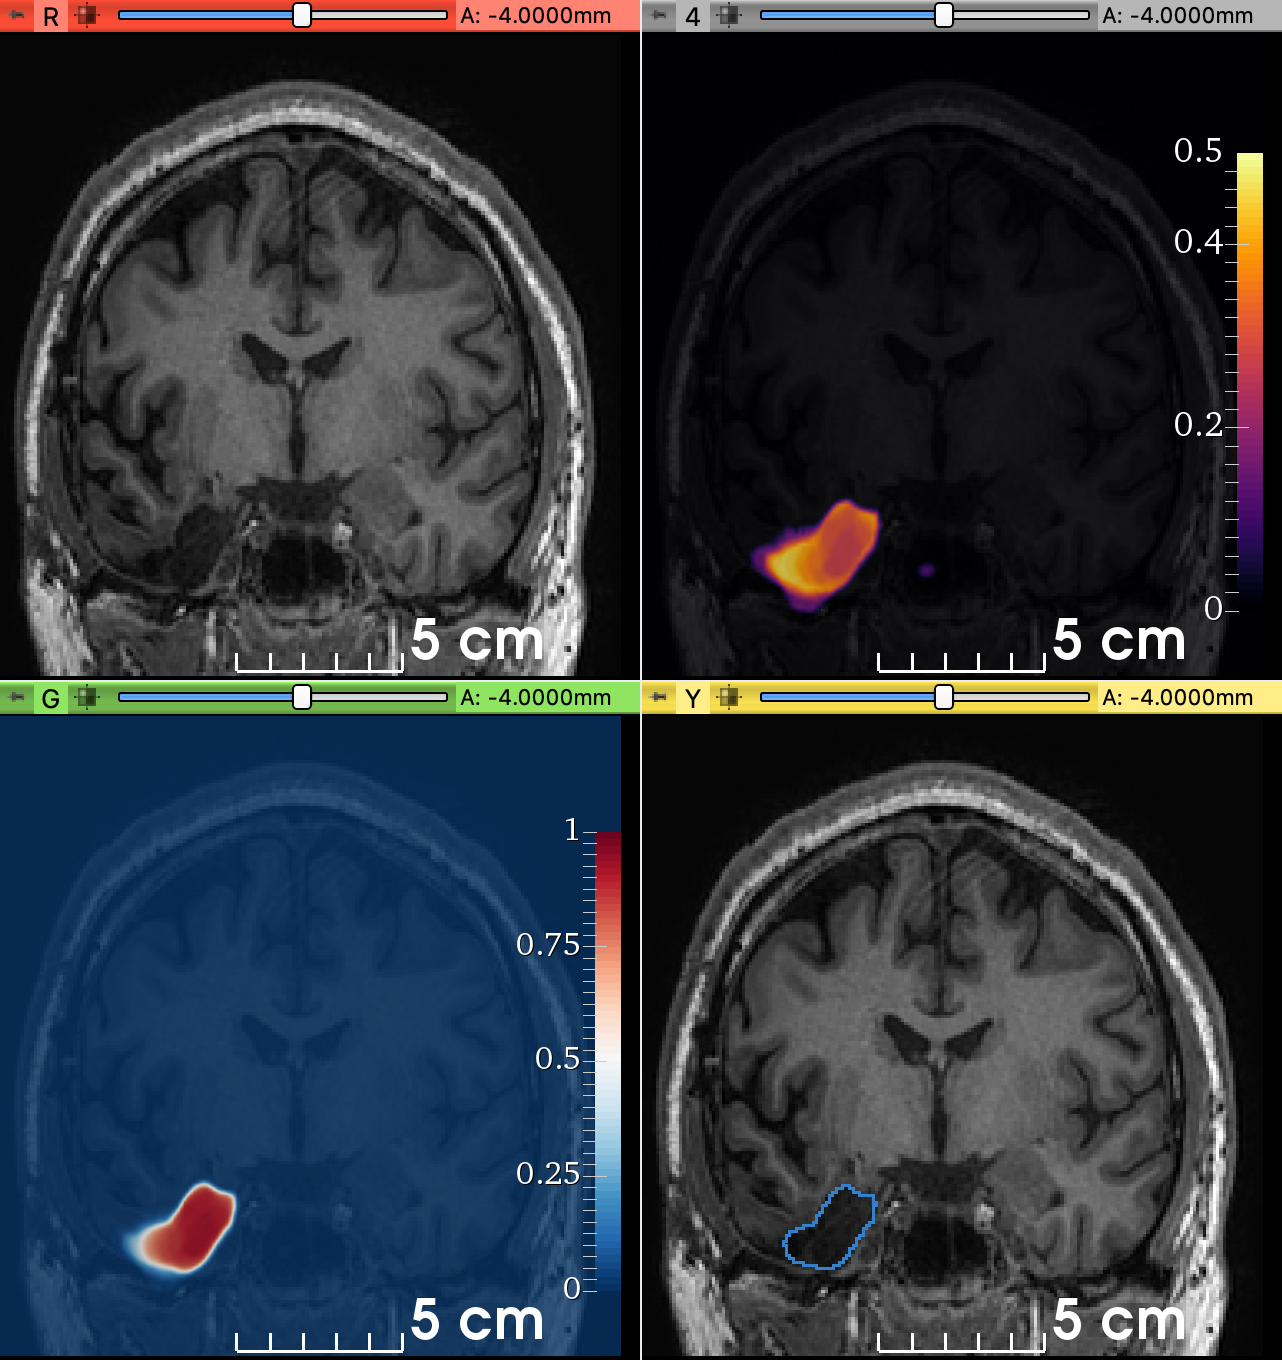
\includegraphics[trim=642 680 0 32, clip, width=0.15\linewidth]{0914_uncertainty} \\
                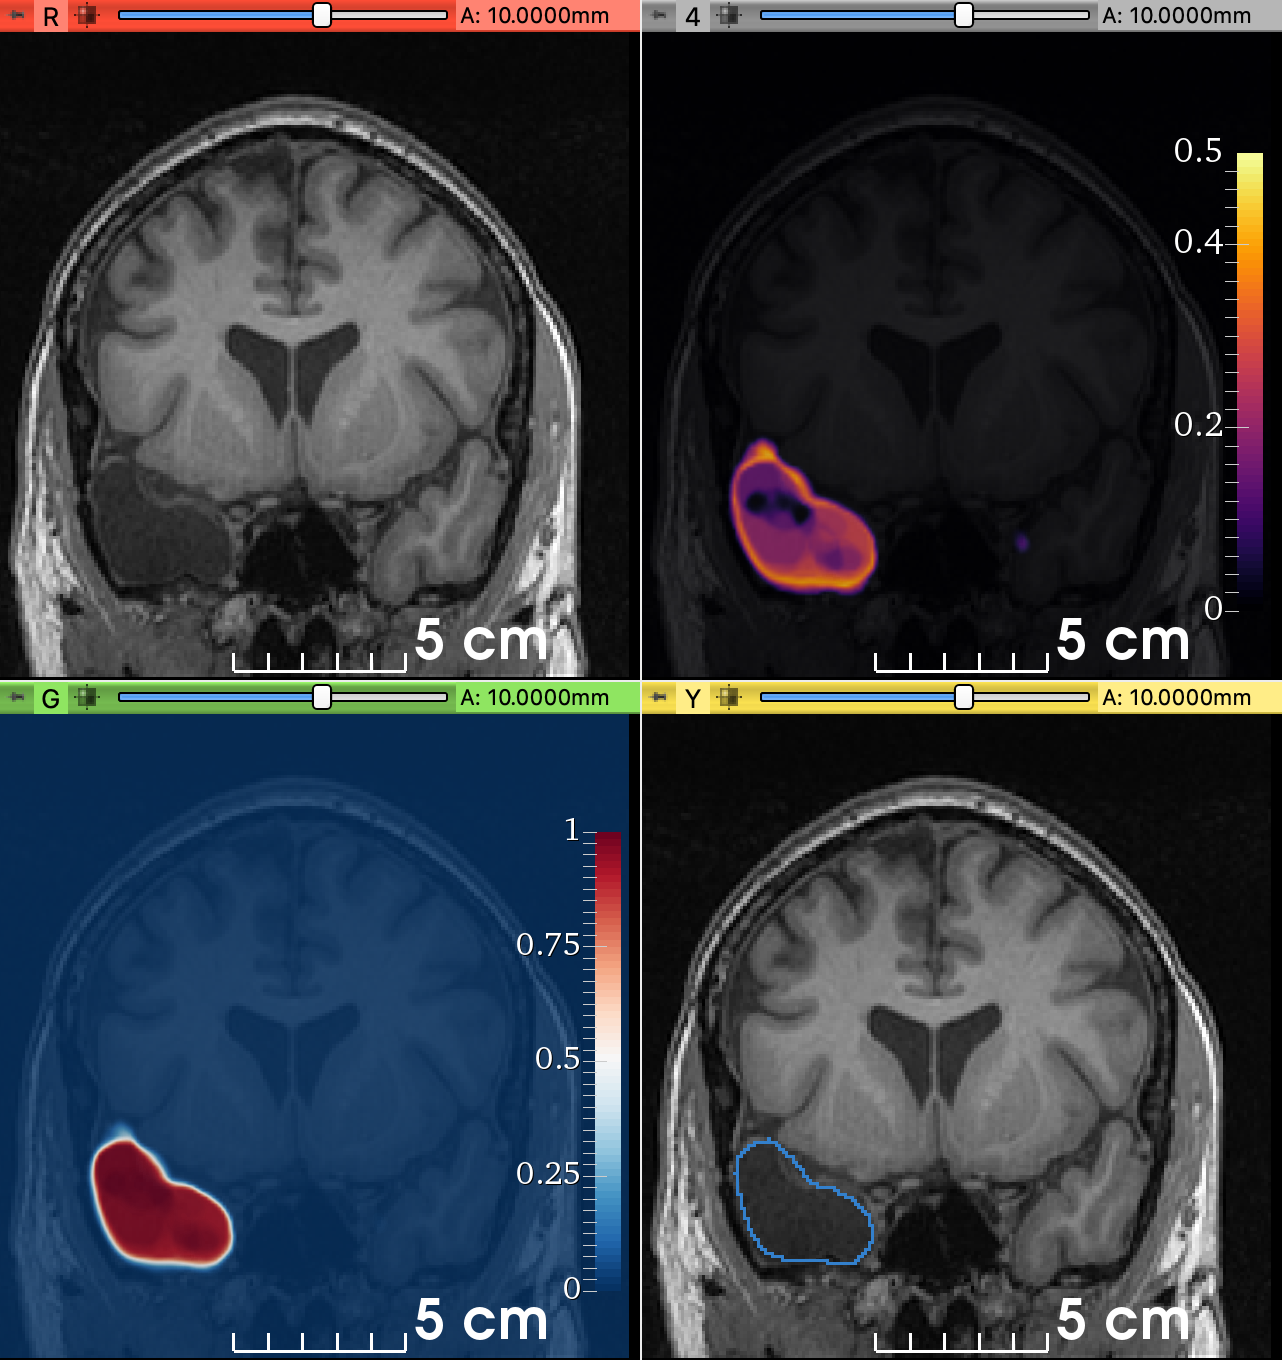
\includegraphics[trim=642 680 0 32, clip, width=0.15\linewidth]{0499_uncertainty} \\
            \end{tabular}
        }%
        \subfigure{%
            \label{fig:uncertainty_mean}%
            \begin{tabular}{c}
                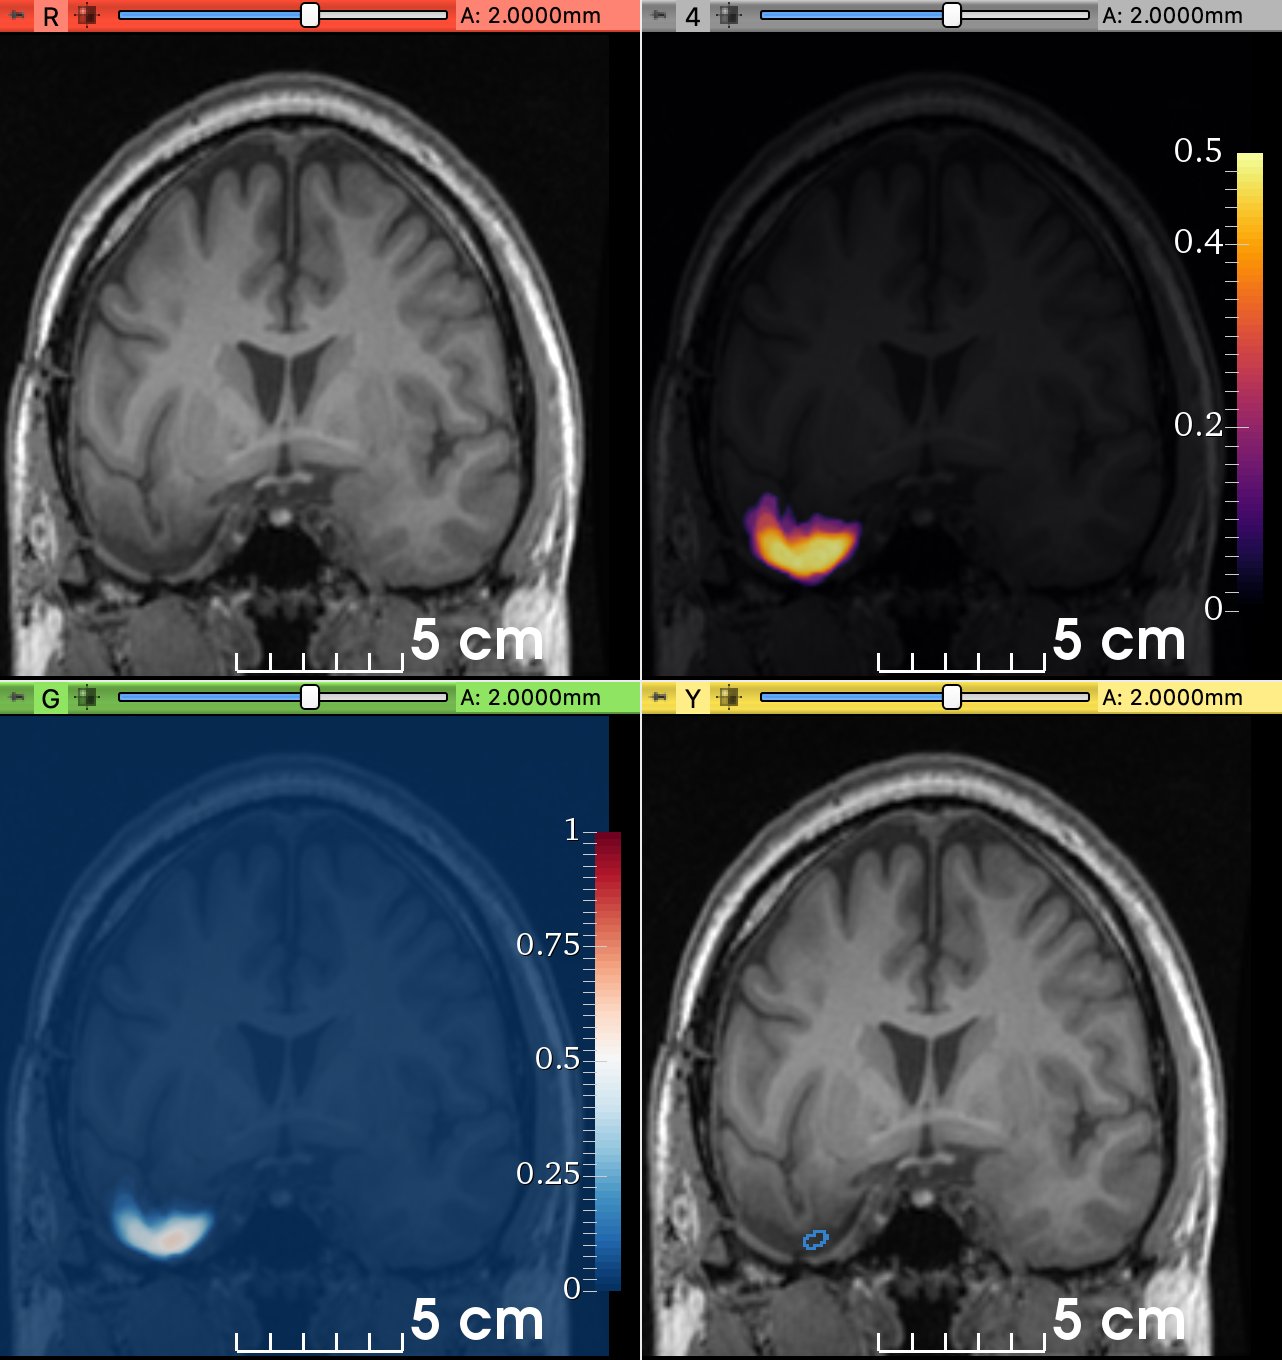
\includegraphics[trim=0 0 642 714, clip, width=0.15\linewidth]{0796_uncertainty} \\
                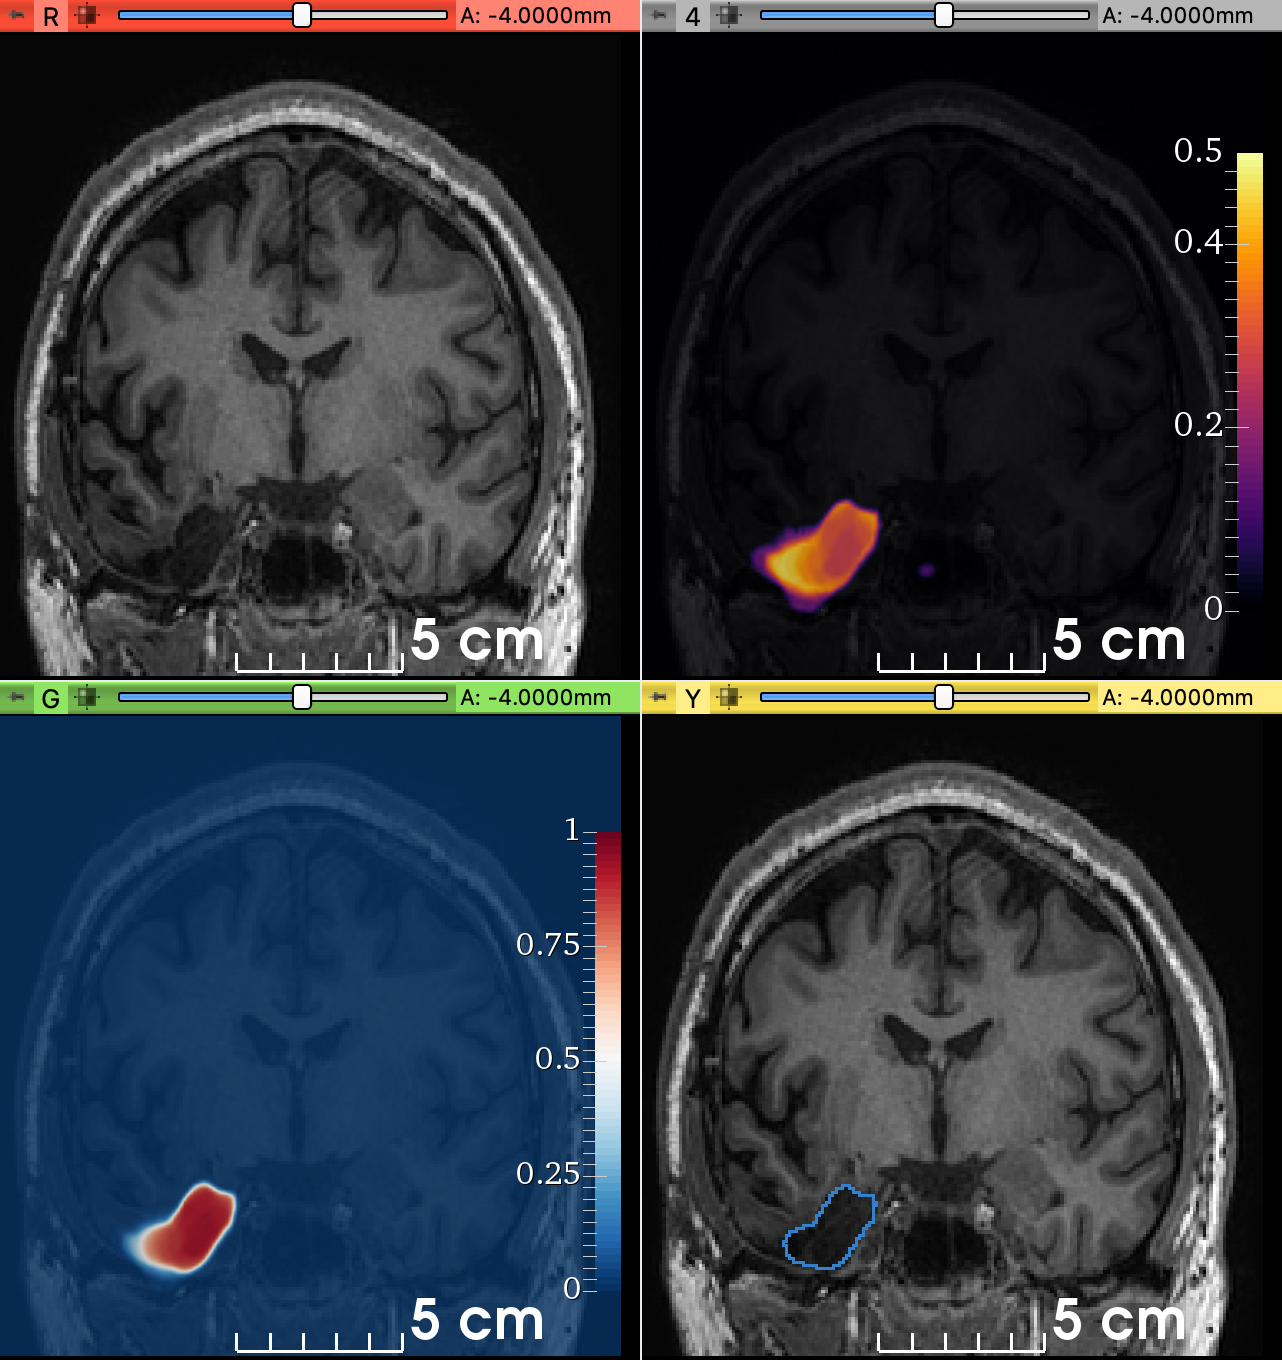
\includegraphics[trim=0 0 642 714, clip, width=0.15\linewidth]{0914_uncertainty} \\
                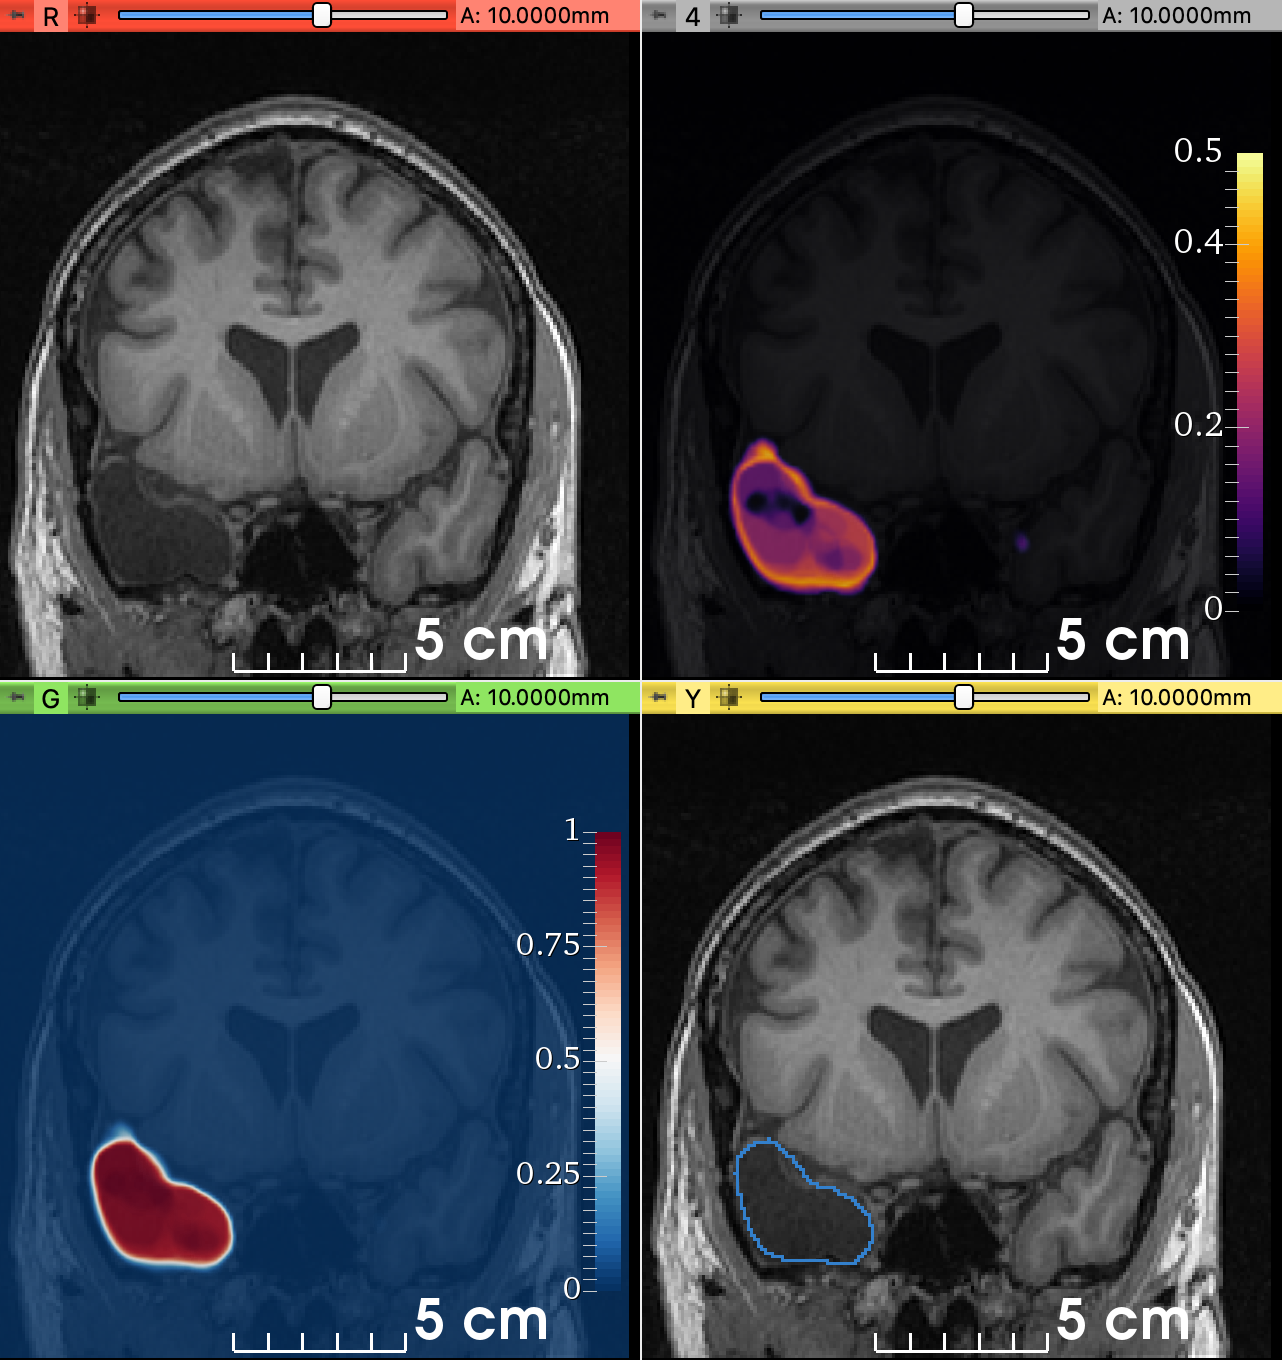
\includegraphics[trim=0 0 642 714, clip, width=0.15\linewidth]{0499_uncertainty} \\
            \end{tabular}
        }%
        \subfigure{%
            \label{fig:uncertainty_pseudo}%
            \begin{tabular}{c}
                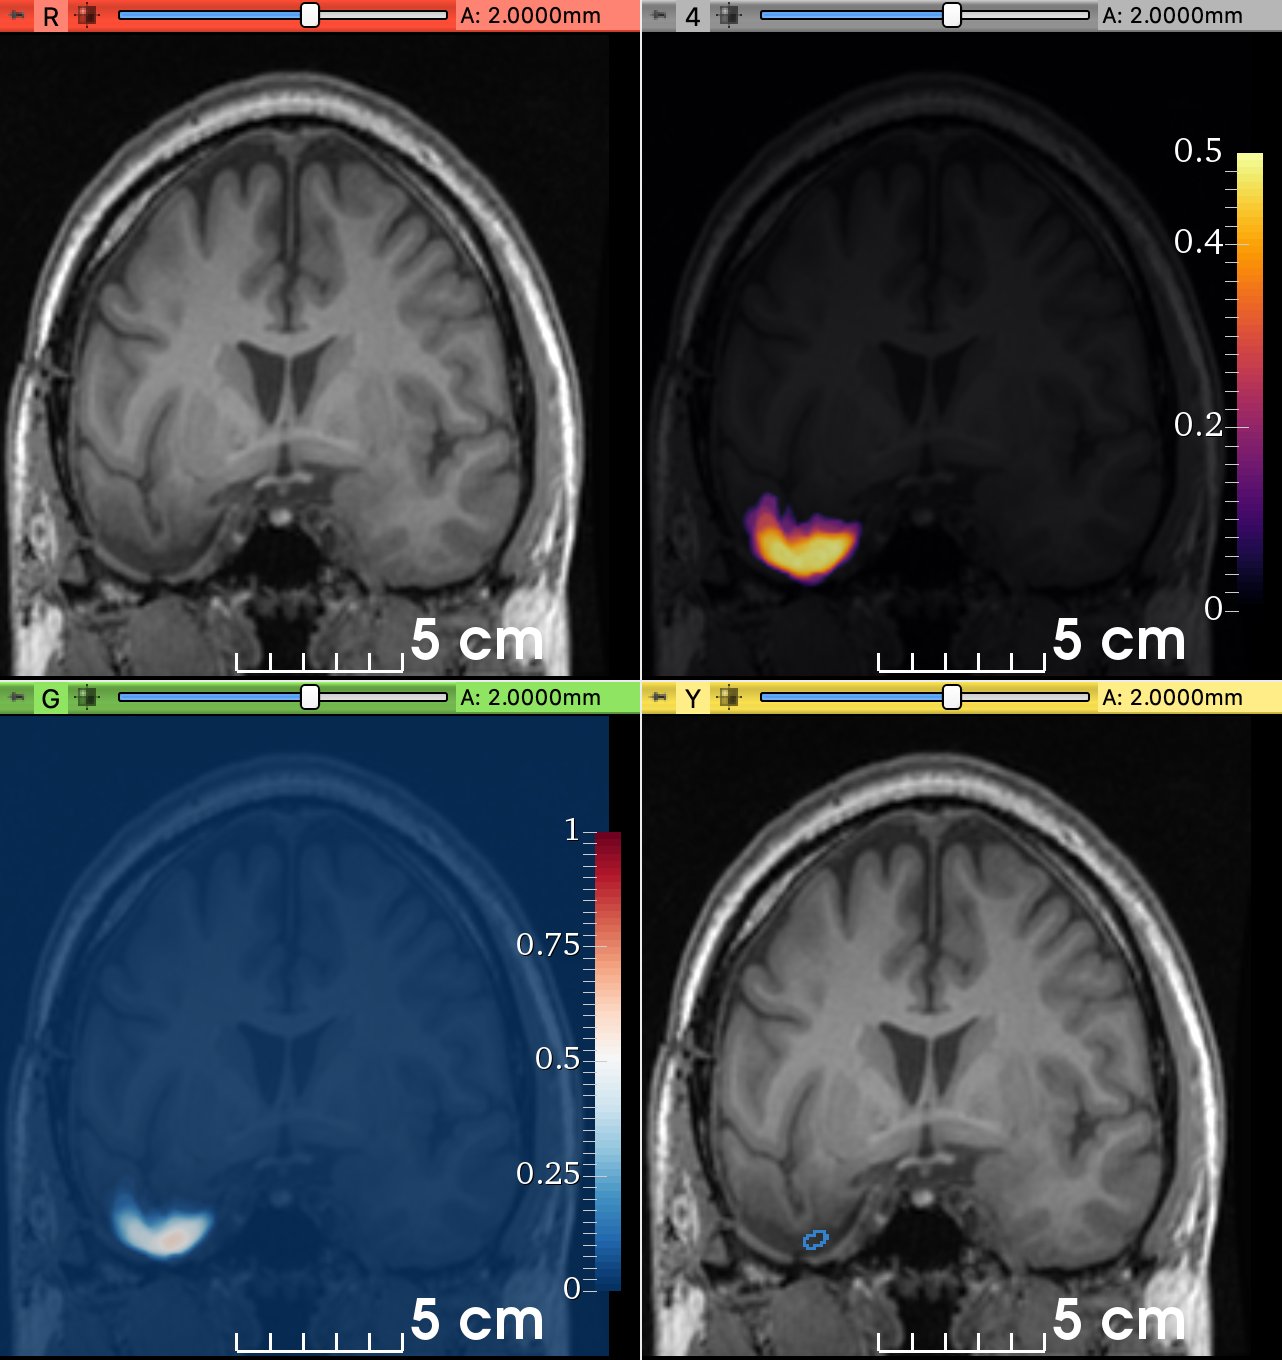
\includegraphics[trim=642 0 0 714, clip, width=0.15\linewidth]{0796_uncertainty} \\
                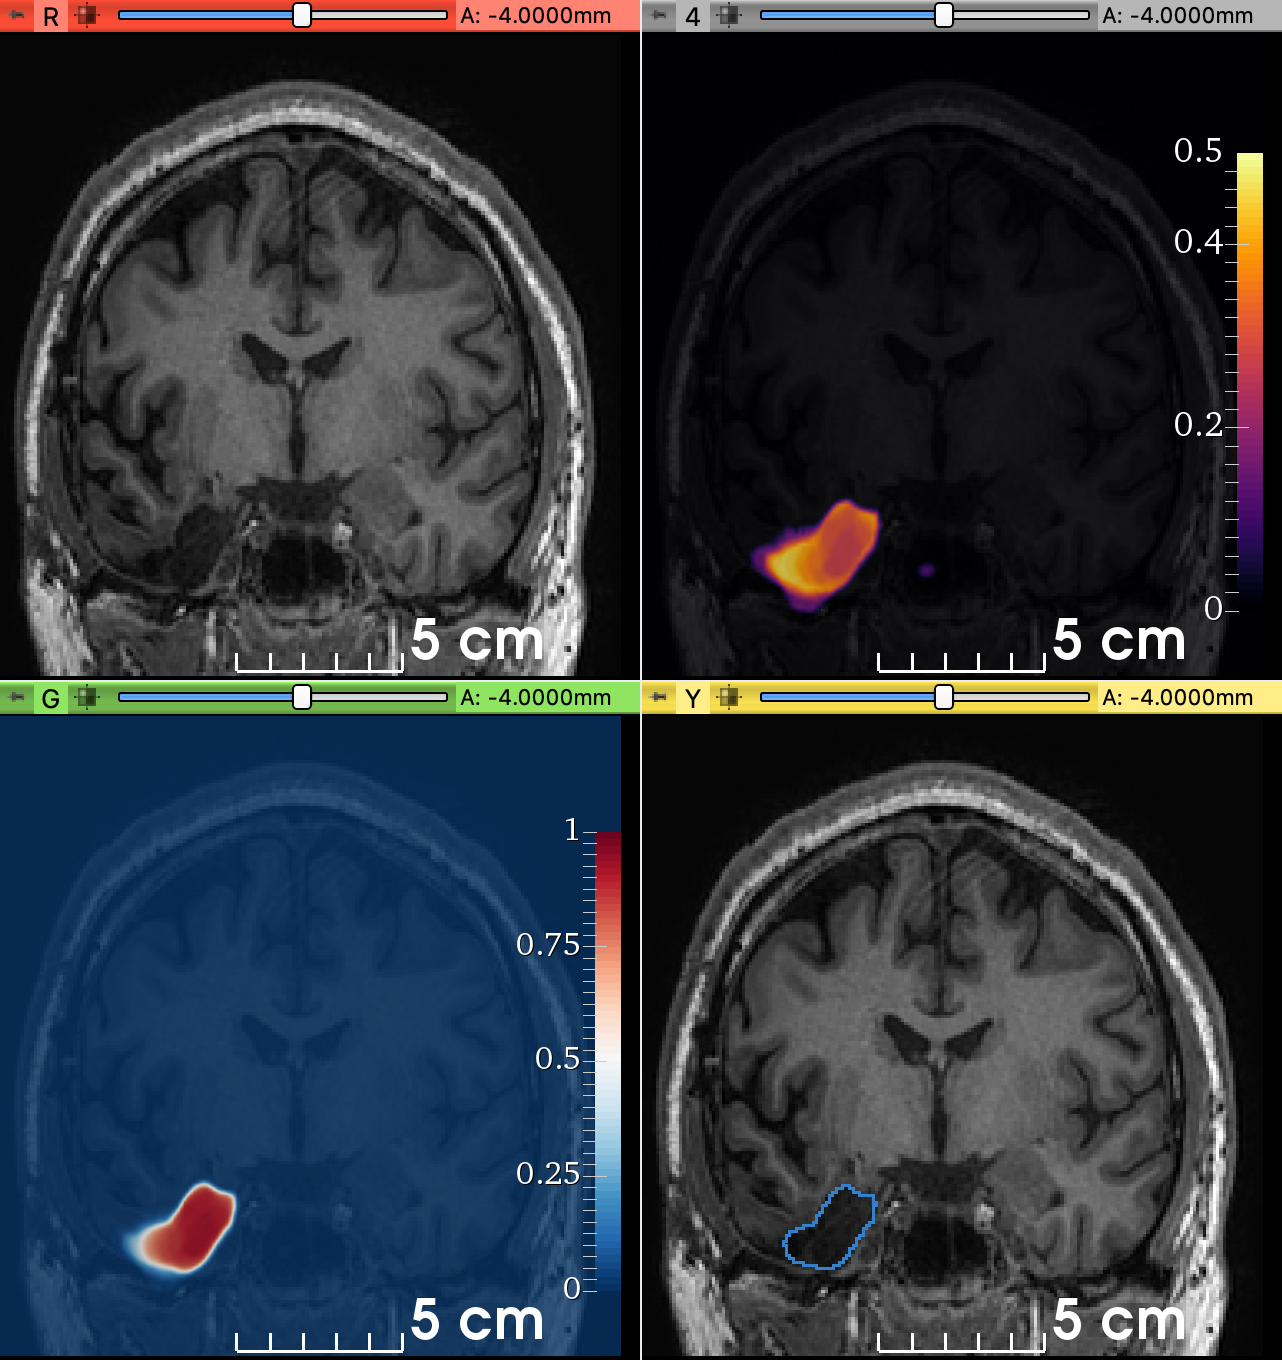
\includegraphics[trim=642 0 0 714, clip, width=0.15\linewidth]{0914_uncertainty} \\
                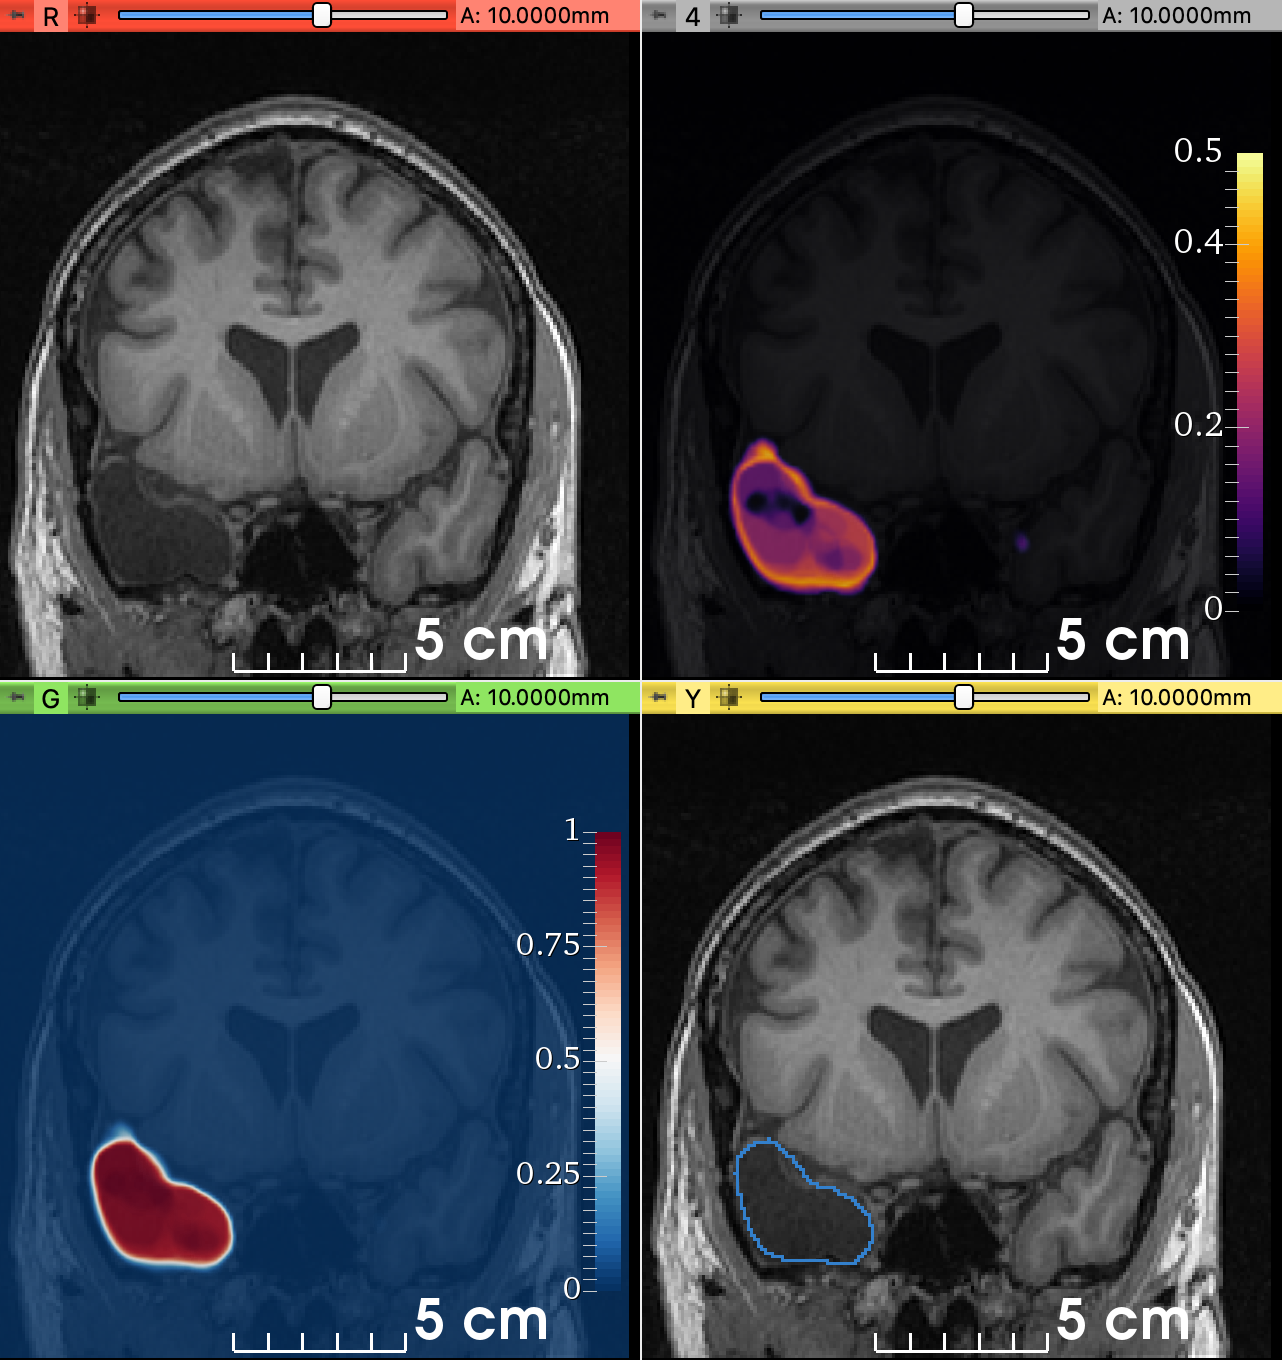
\includegraphics[trim=642 0 0 714, clip, width=0.15\linewidth]{0499_uncertainty} \\
            \end{tabular}
        }
    }
\end{figure}



% \begin{table}
%     \centering
%     \caption{%
%         Results of finetuning the semi-supervised learning model (trained with simulated resection and pseudolabeled images) on EPISURG subsets using 5-fold cross validation (CV).
%     }
%     \label{tab:semi_finetune}
%     \begin{tabular}{l*3c}
%         \toprule
%         \textbf{Dataset}    & \textbf{Subjects} & \textbf{SelfSL \& SemiSL} & \textbf{Finetuning} \\
%         \midrule
%         \textbf{EPISURG (worst)} &           20 &                7.4 (52.5) &          47.4 (52.2) \\ % 43  % worse performance than SelfSL??
%         \textbf{EPISURG} &                  133 &               81.5 (17.8) &          xx.x (xx.x) \\ % 44
%         \bottomrule
%     \end{tabular}
% \end{table}


% CUDA_VISIBLE_DEVICES=0,1 python evaluate.py ~/datasets/real/london_worst/image ~/datasets/real/london_worst/label runs/37/checkpoint.pth /tmp/london_worst_semi_tmp landmarks/histogram_landmarks_default.npy /tmp/london_worst_semi_tmp/eval.csv